\documentclass[a4paper,14pt]{extarticle}

\usepackage[utf8x]{inputenc}
\usepackage[T1,T2A]{fontenc}
\usepackage[russian]{babel}
\usepackage{hyperref}
\usepackage{indentfirst}
\usepackage{here}
\usepackage{array}
\usepackage[table]{xcolor}
\usepackage{datetime}
\usepackage{multirow}
\usepackage{hhline}
\usepackage{mathtools,cancel}
\usepackage{forest}
\usepackage{graphicx}
\usepackage{caption}
\usepackage{subcaption}
\usepackage{chngcntr}
\usepackage{amsmath}
\usepackage{amssymb}
\usepackage{pgfplots}
\usepackage{pgfplotstable}
\usepackage[left=2cm,right=2cm,top=2cm,bottom=2cm,bindingoffset=0cm]{geometry}
\usepackage{multicol}
\usepackage{askmaps}
\usepackage{tikz}

\newcommand*\circled[1]{\tikz[baseline=(char.base)]{
            \node[shape=circle,draw,inner sep=2pt] (char) {#1};}}

\DeclareMathOperator*{\argmin}{argmin}

\renewcommand{\not}[1]{\mkern 1.5mu\overline{\mkern-1.5mu#1\mkern-1.5mu}\mkern 1.5mu}
\renewcommand{\le}{\ensuremath{\leqslant}}
\renewcommand{\leq}{\ensuremath{\leqslant}}
\renewcommand{\ge}{\ensuremath{\geqslant}}
\renewcommand{\geq}{\ensuremath{\geqslant}}
\renewcommand{\epsilon}{\ensuremath{\varepsilon}}
\renewcommand{\phi}{\ensuremath{\varphi}}

\counterwithin{figure}{section}
\counterwithin{equation}{section}
\counterwithin{table}{section}
\newcommand{\sign}[1][5cm]{\makebox[#1]{\hrulefill}} % Поля подписи и даты
\graphicspath{{pics/}} % Путь до папки с картинками
\captionsetup{justification=centering,margin=1cm}
\def\arraystretch{1.3}

\begin{document}

\begin{titlepage}
\begin{center}
	Санкт-Петербургский политехнический университет Петра Великого\\[0.3cm]
	Институт компьютерных наук и технологий \\[0.3cm]
	Кафедра компьютерных систем и программных технологий\\[4cm]
	
	\textbf{Расчётное задание №6}\\[2mm]
	\textbf{Дисциплина:} Системный анализ и принятие решений\\[2mm]
	\textbf{Тема:} Дискретное программирование. Задача коммивояжёра\\[2mm]
	Вариант 39\\[6.5cm]
\end{center}

\begin{flushleft}
	\hspace*{5mm} Выполнил студент гр. 33501/4  \hspace*{3cm}\sign[3cm]\hspace*{2mm} А.Ю. Ламтев\\
	\hspace*{10.85cm} (подпись)\\[2.5mm]
	\hspace*{5mm} Преподаватель \hspace*{6.45cm}\sign[3cm]\hspace*{2mm} С.С. Сабонис\\
	\hspace*{10.85cm} (подпись)\\[2.5mm]
	\hspace*{11.1cm} <<\underline{\the\day}>> \underline{\hspace{5mm}ноября\hspace{5mm}} \the\year\hspace{1mm} г.
\end{flushleft}

\vfill

\begin{center}
	Санкт-Петербург\\
	\the\year
\end{center}
\end{titlepage}
\addtocounter{page}{1}

\section{Задание}

\begin{figure}[H]
\begin{center}
	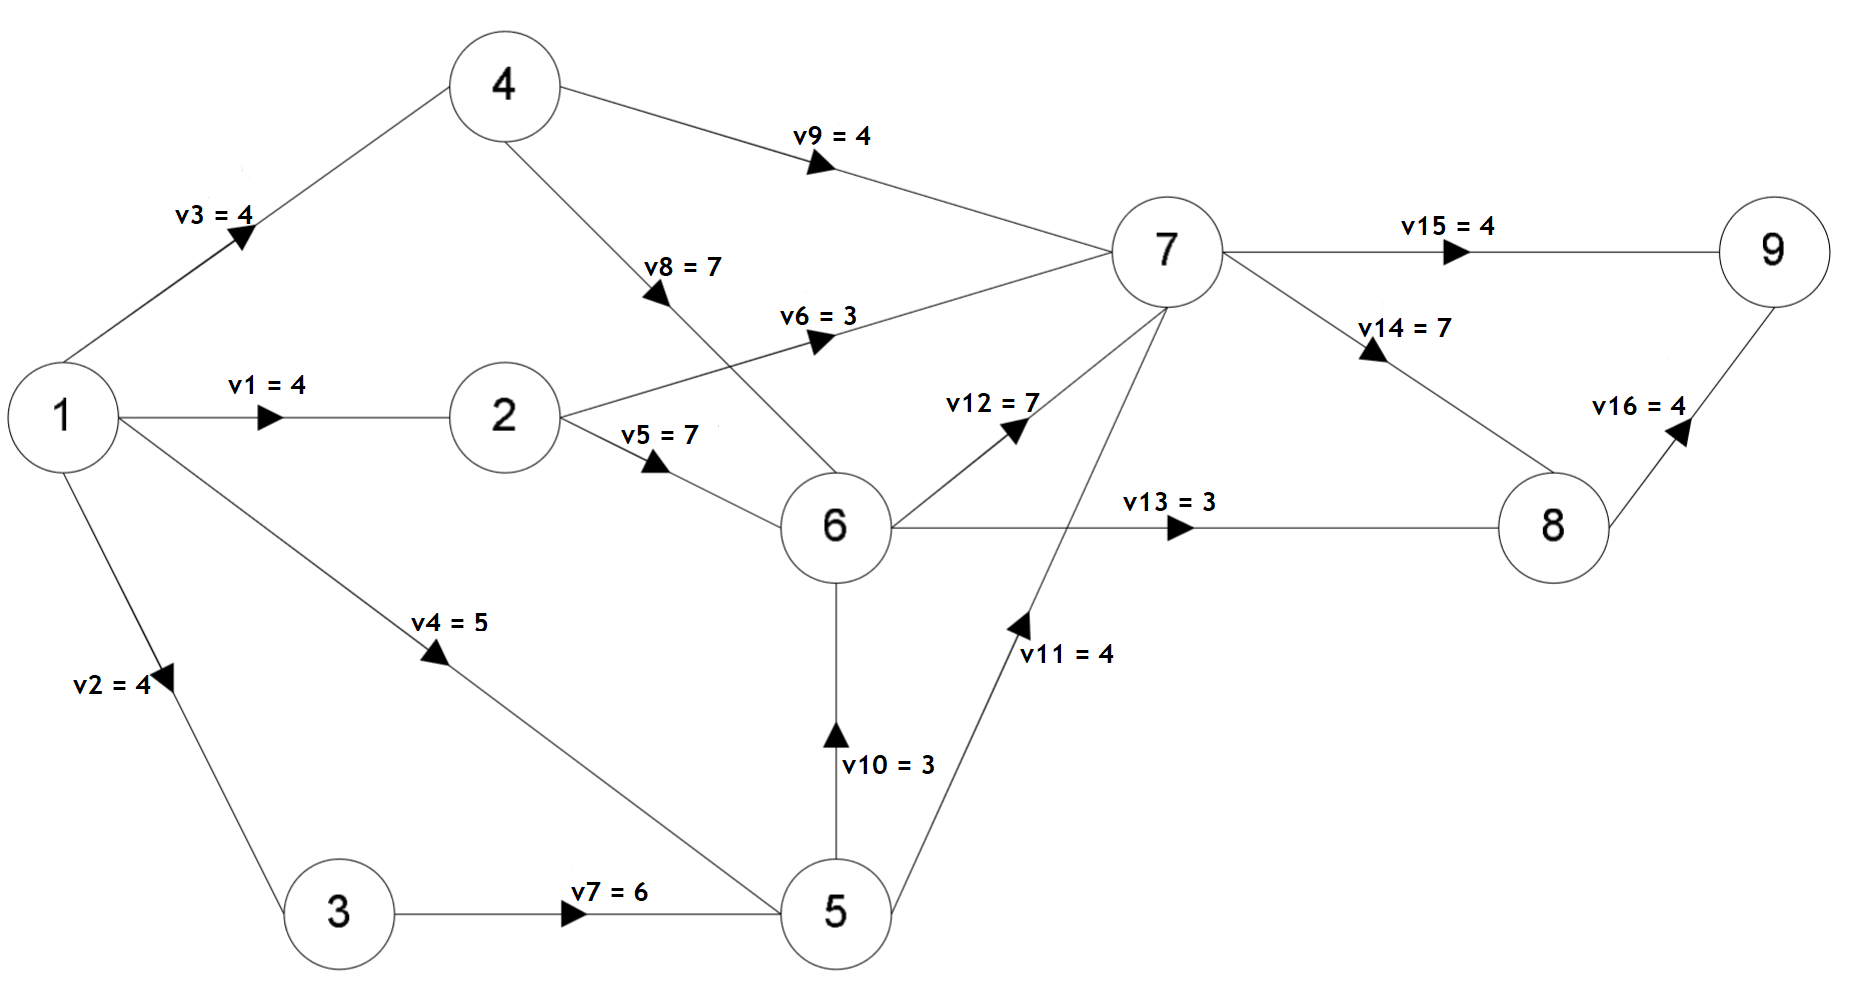
\includegraphics[width=1\textwidth]{graph-src}
	\caption{Исходный ориентрированный граф}
	\label{pic:graph-src}
\end{center}
\end{figure}

На основе графа, изображенного на рис. \ref{pic:graph-src}:

\begin{enumerate}
\item Написать матрицу смежности
\item Определить наиболее ранние моменты наступления событий
\item Определить наиболее поздние моменты наступления событий
\item Определить резервы времени, написать матрицу резервов
\item Найти критический путь
\item Определить минимально возможное время выполнения всего комплекса работ
\item Для $n = 1$ определить время выполнения всего комплекса работ
\item Для $n = 2$ найти распределение работ по ресурсам, рассмотреть 4 критерия выбора работ для выполнения: 
\begin{itemize}
\item работа наименьшей длительности
\item работа наибольшей длительности
\item работа с наименьшим резервом
\item работа с наибольшим резервом
\end{itemize}. 
Для каждого критерия:

\begin{itemize}
\item привести решение задачи по шагам
\item построить график
\item найти общее время работы
\item найти времена простоя каждого ресурса
\end{itemize}
Из полученных расписаний выбрать наилучшее.

\end{enumerate}

\section{Решение}

\subsection{Часть 1}

Для заданного графа составим матрицу смежности. Она представлена в таблице \ref{tab:smezhnost}.

\begin{table}[H]
\begin{center}
	\def\tabcolsep{8pt}
	\caption{Матрица смежности}
	\label{tab:smezhnost}
	\begin{tabular}{|c|c|c|c|c|c|c|c|c|c|}
	\hline 
	 & 1 & 2 & 3 & 4 & 5 & 6 & 7 & 8 & 9 \\ 
	\hline 
	1 &  & 4 & 4 & 4 & 5 &  &  &  &  \\ 
	\hline 
	2 &  &  &  &  &  & 7 & 3 &  &  \\ 
	\hline 
	3 &  &  &  &  & 6 &  &  &  &  \\ 
	\hline 
	4 &  &  &  &  &  & 7 & 4 &  &  \\ 
	\hline 
	5 &  &  &  &  &  & 3 & 4 &  &  \\ 
	\hline 
	6 &  &  &  &  &  &  & 7 & 3 &  \\ 
	\hline 
	7 &  &  &  &  &  &  &  & 7 & 4 \\ 
	\hline 
	8 &  &  &  &  &  &  &  &  & 4 \\ 
	\hline 
	9 &  &  &  &  &  &  &  &  &  \\ 
	\hline 
	\end{tabular} 
\end{center}
\end{table}

Вычислим наиболее ранние и наиболее поздние моменты наступления событий, которые определяются по формулам \ref{eq:early} и \ref{eq:late} соответственно. Они представлены в таблице \ref{tab:earlylate}.

\begin{equation}
\label{eq:early}
	t^{'}_i = max (t^{'}_j + \tau_{ji}),\ j \in G^-(i)
\end{equation}

\begin{equation}
\label{eq:late}
	t^{''}_j = max (t^{''}_ij + \tau_{ji}),\ i \in G(i)
\end{equation}

где $\tau_{ji}$ --- время выполнения работы для перехода между событиями $j$ и $i$, а $G$ и $G^{-}$ ---  множества прямого и обратного соответствия.

\begin{table}[H]
\begin{center}
	\def\tabcolsep{8pt}
	\caption{Наиболее ранние и наиболее поздние моменты наступления событий}
	\label{tab:earlylate}
	\begin{tabular}{|c|c|c|c|c|c|c|c|c|c|}
	\hline 
	$i$ & 1 & 2 & 3 & 4 & 5 & 6 & 7 & 8 & 9 \\ 
	\hline 
	$t^{'}_i$ & 0 & 4 & 4 & 4 & 10 & 13 & 20 & 27 & 31 \\ 
	\hline 
	$t^{''}_i$ & 0 & 6 & 4 & 6 & 10 & 13 & 20 & 27 & 31 \\ 
	\hline 
	\end{tabular}  
\end{center}
\end{table}

Определим резервы времени и запишем их в матрицу, изображенную в таблице \ref{tab:reserv}.

\begin{table}[H]
\begin{center}
	\def\tabcolsep{8pt}
	\caption{Матрица резервов времени}
	\label{tab:reserv}
	\begin{tabular}{|c|c|c|c|c|c|c|c|c|c|}
	\hline 
	 & 1 & 2 & 3 & 4 & 5 & 6 & 7 & 8 & 9 \\ 
	\hline 
	1 &  & 2 & 0 & 2 & 5  &  &  &  &  \\ 
	\hline 
	2 &  &  &  &  &  & 2 & 13  &  &  \\ 
	\hline 
	3 &  &  &  &  & 0 &  &  &  &  \\ 
	\hline 
	4 &  &  &  &  &  & 2 & 12 &  &  \\ 
	\hline 
	5 &  &  &  &  &  & 0 & 6 &  &  \\ 
	\hline 
	6 &  &  &  &  &  &  & 0 & 11 &  \\ 
	\hline 
	7 &  &  &  &  &  &  &  & 0 & 7 \\ 
	\hline 
	8 &  &  &  &  &  &  &  &  & 0 \\ 
	\hline 
	9 &  &  &  &  &  &  &  &  &  \\ 
	\hline 
	\end{tabular} 
\end{center}
\end{table}

Критический путь: $1 \rightarrow 3 \rightarrow 5 \rightarrow 6 \rightarrow 7 \rightarrow 8 \rightarrow 9$ длиной в 31.

Минимально возможное время выполнения всего комплекса работ: 76.

\subsection{Часть 2}

Для числа рабочих $n = 1$ время выполнения всего комплекса работ --- это сумма времени выполнения всех работ, т.е. 76.

Для числа рабочих $n = 2$ найдём распределение работ по
ресурсам, рассмотрим 4 критерия выбора работ для выполнения.

\paragraph{$max\ A$} Решим задачу по шагам. Решение представлено в таблице \ref{tab:maxa}.

\begin{table}[H]
\begin{center}
	\def\tabcolsep{2pt}
	\caption{Пошаговое решение. Критерий $max\ A$}
	\label{tab:maxa}
	\begin{tabular}{|c|c|c|c|c|c|c|c|c|c|}
	\hline 
	T & D & E & W & A & B & L\\ \hline
	0 & [~] & [0] & [0 1] [0 2] [0 3] [0 4] & [4 4 4 5] & [0 4] [0 1] & [5 4] \\ \hline
4 & [0 1] & [0 1] & [0 2] [0 3] [1 5] [1 6] & [4 4 7 3] & [0 4] [1 5] & [1 7] \\ \hline
5 & [0 4] & [0 1] & [0 2] [0 3] [1 6] & [4 4 3] & [1 5] [0 2] & [6 4] \\ \hline
9 & [0 2] & [0 1 2] & [0 3] [1 6] [2 4] & [4 3 6] & [1 5] [2 4] & [2 6] \\ \hline
11 & [1 5] & [0 1 2] & [0 3] [1 6] & [4 3] & [2 4] [0 3] & [4 4] \\ \hline
15 & [2 4] [0 3] & [0 1 2 3 4] & [1 6] [3 5] [3 6] [4 5] [4 6] & [3 7 4 3 4] & [3 5] [3 6] & [7 4] \\ \hline
19 & [3 6] & [0 1 2 3 4] & [1 6] [4 5] [4 6] & [3 3 4] & [3 5] [4 6] & [3 4] \\ \hline
22 & [3 5] & [0 1 2 3 4] & [1 6] [4 5] & [3 3] & [4 6] [1 6] & [1 3] \\ \hline
23 & [4 6] & [0 1 2 3 4] & [4 5] & [3] & [1 6] [4 5] & [2 3] \\ \hline
25 & [1 6] & [0 1 2 3 4] & [~] & [~] & [4 5] & [1] \\ \hline
26 & [4 5] & [0 1 2 3 4 5] & [5 6] [5 7] & [7 3] & [5 6] [5 7] & [7 3] \\ \hline
29 & [5 7] & [0 1 2 3 4 5] & [~] & [~] & [5 6] & [4] \\ \hline
33 & [5 6] & [0 1 2 3 4 5 6] & [6 7] [6 8] & [7 4] & [6 7] [6 8] & [7 4] \\ \hline
37 & [6 8] & [0 1 2 3 4 5 6] & [~] & [~] & [6 7] & [3] \\ \hline
40 & [6 7] & [0 1 2 3 4 5 6 7] & [7 8] & [4] & [7 8] & [4] \\ \hline
44 & [7 8] & [0 1 2 3 4 5 6 7 8] & [~] & [~] & [~] & [~] \\ \hline
	\end{tabular} 
\end{center}
\end{table}

На рис. \ref{pic:diag1} изображена диаграмма распределения работ по ресурсам.

\begin{figure}[H]
\begin{center}
	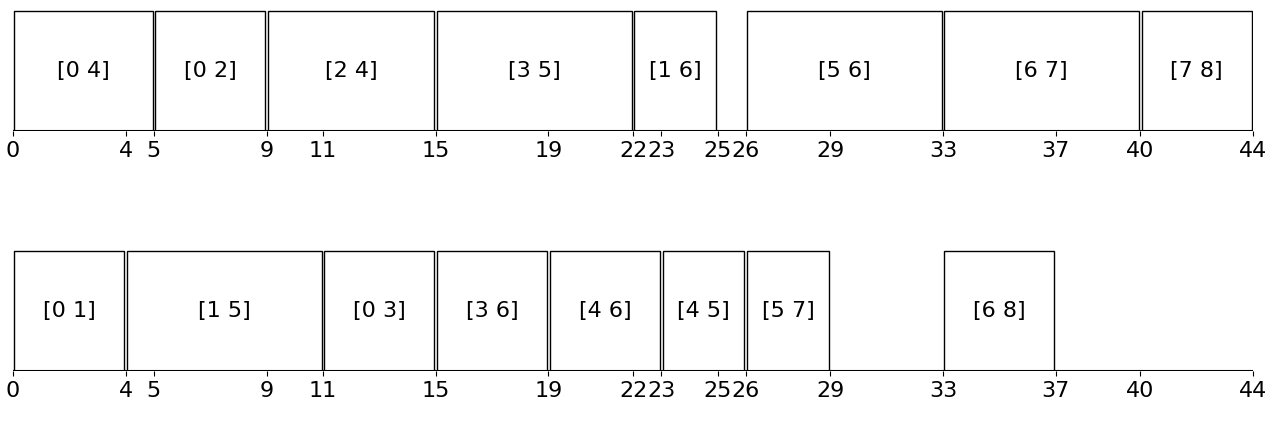
\includegraphics[width=0.95\textwidth]{diag1}
	\caption{Диаграмма Ганта. Критерий $max\ A$}
	\label{pic:diag1}
\end{center}
\end{figure}

Общее время работы: 44 часа.\  1-й простаивал 1 час, 2-й --- 11 часов.

\paragraph{$min\ A$} Решим задачу по шагам. Решение представлено в таблице \ref{tab:mina}.

\begin{table}[H]
\begin{center}
	\def\tabcolsep{2pt}
	\caption{Пошаговое решение. Критерий $min\ A$}
	\label{tab:mina}
	\begin{tabular}{|c|c|c|c|c|c|c|c|c|c|}
	\hline 
	T & D & E & W & A & B & L\\ \hline
0 & [~] & [0] & [0 1] [0 2] [0 3] [0 4] & [4 4 4 5] & [0 1] [0 2] & [4 4] \\ \hline
4 & [0 1] [0 2] & [0 1 2] & [0 3] [0 4] [1 5] [1 6] [2 4] & [4 5 7 3 6] & [1 6] [0 3] & [3 4] \\ \hline
7 & [1 6] & [0 1 2] & [0 4] [1 5] [2 4] & [5 7 6] & [0 3] [0 4] & [1 5] \\ \hline
8 & [0 3] & [0 1 2 3] & [1 5] [2 4] [3 5] [3 6] & [7 6 7 4] & [0 4] [3 6] & [4 4] \\ \hline
12 & [0 4] [3 6] & [0 1 2 3] & [1 5] [2 4] [3 5] & [7 6 7] & [2 4] [1 5] & [6 7] \\ \hline
18 & [2 4] & [0 1 2 3 4] & [3 5] [4 5] [4 6] & [7 3 4] & [1 5] [4 5] & [1 3] \\ \hline
19 & [1 5] & [0 1 2 3 4] & [3 5] [4 6] & [7 4] & [4 5] [4 6] & [2 4] \\ \hline
21 & [4 5] & [0 1 2 3 4] & [3 5] & [7] & [4 6] [3 5] & [2 7] \\ \hline
23 & [4 6] & [0 1 2 3 4] & [~] & [~] & [3 5] & [5] \\ \hline
28 & [3 5] & [0 1 2 3 4 5] & [5 6] [5 7] & [7 3] & [5 7] [5 6] & [3 7] \\ \hline
31 & [5 7] & [0 1 2 3 4 5] & [~] & [~] & [5 6] & [4] \\ \hline
35 & [5 6] & [0 1 2 3 4 5 6] & [6 7] [6 8] & [7 4] & [6 8] [6 7] & [4 7] \\ \hline
39 & [6 8] & [0 1 2 3 4 5 6] & [~] & [~] & [6 7] & [3] \\ \hline
42 & [6 7] & [0 1 2 3 4 5 6 7] & [7 8] & [4] & [7 8] & [4] \\ \hline
46 & [7 8] & [0 1 2 3 4 5 6 7 8] & [~] & [~] & [~] & [~] \\ \hline
	\end{tabular} 
\end{center}
\end{table}

На рис. \ref{pic:diag2} изображена диаграмма распределения работ по ресурсам.

\begin{figure}[H]
\begin{center}
	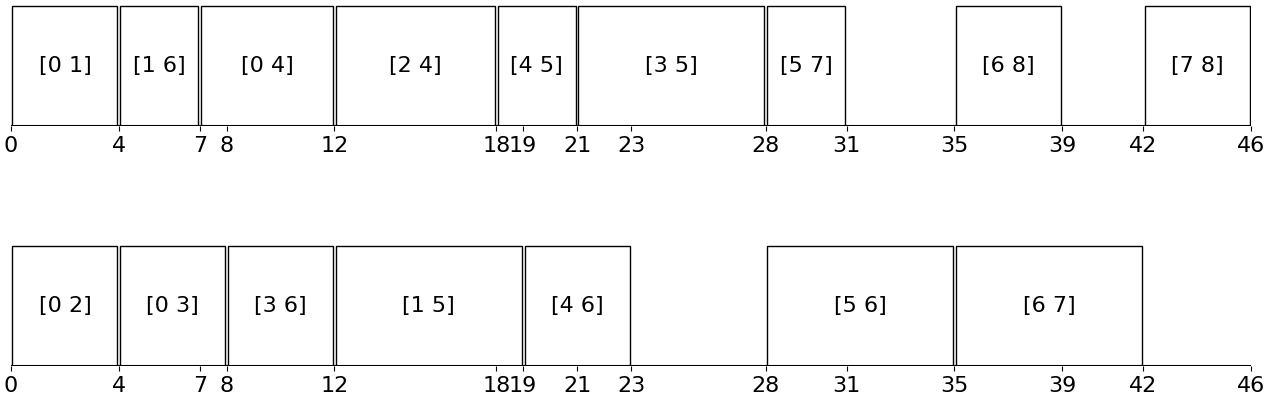
\includegraphics[width=0.95\textwidth]{diag2}
	\caption{Диаграмма Ганта. Критерий $min\ A$}
	\label{pic:diag2}
\end{center}
\end{figure}

Общее время работы: 46 часов.\  1-й простаивал 7 часов, 2-й --- 9 часов.

\paragraph{$min\ R$} Решим задачу по шагам. Решение представлено в таблице \ref{tab:minr}.

\begin{table}[H]
\begin{center}
	\def\tabcolsep{2pt}
	\caption{Пошаговое решение. Критерий $min\ R$}
	\label{tab:minr}
	\begin{tabular}{|c|c|c|c|c|c|c|c|c|c|}
	\hline 
	T & D & E & W & A & B & L\\ \hline
0 & [~] & [0] & [0 1] [0 2] [0 3] [0 4] & [4 4 4 5] & [0 4] [0 1] & [5 4] \\ \hline
4 & [0 1] & [0 1] & [0 2] [0 3] [1 5] [1 6] & [4 4 7 3] & [0 4] [1 6] & [1 3] \\ \hline
5 & [0 4] & [0 1] & [0 2] [0 3] [1 5] & [4 4 7] & [1 6] [0 3] & [2 4] \\ \hline
7 & [1 6] & [0 1] & [0 2] [1 5] & [4 7] & [0 3] [1 5] & [2 7] \\ \hline
9 & [0 3] & [0 1 3] & [0 2] [3 5] [3 6] & [4 7 4] & [1 5] [3 6] & [5 4] \\ \hline
13 & [3 6] & [0 1 3] & [0 2] [3 5] & [4 7] & [1 5] [3 5] & [1 7] \\ \hline
14 & [1 5] & [0 1 3] & [0 2] & [4] & [3 5] [0 2] & [6 4] \\ \hline
18 & [0 2] & [0 1 2 3] & [2 4] & [6] & [3 5] [2 4] & [2 6] \\ \hline
20 & [3 5] & [0 1 2 3] & [~] & [~] & [2 4] & [4] \\ \hline
24 & [2 4] & [0 1 2 3 4] & [4 5] [4 6] & [3 4] & [4 6] [4 5] & [4 3] \\ \hline
27 & [4 5] & [0 1 2 3 4 5] & [5 6] [5 7] & [7 3] & [4 6] [5 7] & [1 3] \\ \hline
28 & [4 6] & [0 1 2 3 4 5] & [5 6] & [7] & [5 7] [5 6] & [2 7] \\ \hline
30 & [5 7] & [0 1 2 3 4 5] & [~] & [~] & [5 6] & [5] \\ \hline
35 & [5 6] & [0 1 2 3 4 5 6] & [6 7] [6 8] & [7 4] & [6 8] [6 7] & [4 7] \\ \hline
39 & [6 8] & [0 1 2 3 4 5 6] & [~] & [~] & [6 7] & [3] \\ \hline
42 & [6 7] & [0 1 2 3 4 5 6 7] & [7 8] & [4] & [7 8] & [4] \\ \hline
46 & [7 8] & [0 1 2 3 4 5 6 7 8] & [~] & [~] & [~] & [~] \\ \hline
	\end{tabular} 
\end{center}
\end{table}

На рис. \ref{pic:diag3} изображена диаграмма распределения работ по ресурсам.

Общее время работы: 46 часов.\  1-й простаивал 7 часов, 2-й --- 9 часов.

\begin{figure}[H]
\begin{center}
	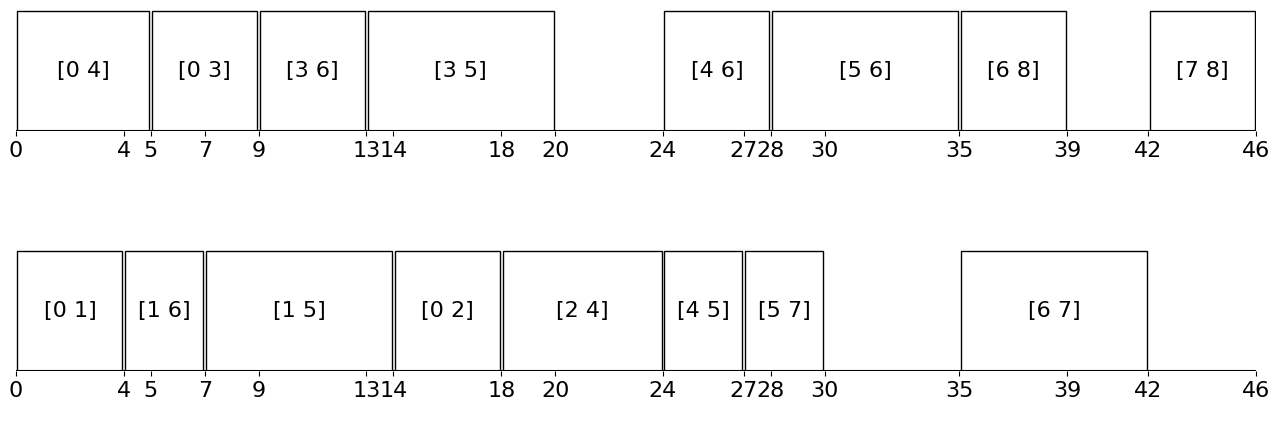
\includegraphics[width=0.95\textwidth]{diag3}
	\caption{Диаграмма Ганта. Критерий $min\ R$}
	\label{pic:diag3}
\end{center}
\end{figure}

\paragraph{$max\ R$} Решим задачу по шагам. Решение представлено в таблице \ref{tab:maxr}.

\begin{table}[H]
\begin{center}
	\def\tabcolsep{2pt}
	\caption{Пошаговое решение. Критерий $max\ R$}
	\label{tab:maxr}
	\begin{tabular}{|c|c|c|c|c|c|c|c|c|c|}
	\hline 
	T & D & E & W & A & B & L\\ \hline
0 & [~] & [0] & [0 1] [0 2] [0 3] [0 4] & [4 4 4 5] & [0 2] [0 1] & [4 4] \\ \hline
4 & [0 2] [0 1] & [0 1 2] & [0 3] [0 4] [1 5] [1 6] [2 4] & [4 5 7 3 6] & [2 4] [0 3] & [6 4] \\ \hline
8 & [0 3] & [0 1 2 3] & [0 4] [1 5] [1 6] [3 5] [3 6] & [5 7 3 7 4] & [2 4] [1 5] & [2 7] \\ \hline
10 & [2 4] & [0 1 2 3] & [0 4] [1 6] [3 5] [3 6] & [5 3 7 4] & [1 5] [3 5] & [5 7] \\ \hline
15 & [1 5] & [0 1 2 3] & [0 4] [1 6] [3 6] & [5 3 4] & [3 5] [0 4] & [2 5] \\ \hline
17 & [3 5] & [0 1 2 3] & [1 6] [3 6] & [3 4] & [0 4] [3 6] & [3 4] \\ \hline
20 & [0 4] & [0 1 2 3 4] & [1 6] [4 5] [4 6] & [3 3 4] & [3 6] [4 5] & [1 3] \\ \hline
21 & [3 6] & [0 1 2 3 4] & [1 6] [4 6] & [3 4] & [4 5] [4 6] & [2 4] \\ \hline
23 & [4 5] & [0 1 2 3 4 5] & [1 6] [5 6] [5 7] & [3 7 3] & [4 6] [5 6] & [2 7] \\ \hline
25 & [4 6] & [0 1 2 3 4 5] & [1 6] [5 7] & [3 3] & [5 6] [5 7] & [5 3] \\ \hline
28 & [5 7] & [0 1 2 3 4 5] & [1 6] & [3] & [5 6] [1 6] & [2 3] \\ \hline
30 & [5 6] & [0 1 2 3 4 5] & [~] & [~] & [1 6] & [1] \\ \hline
31 & [1 6] & [0 1 2 3 4 5 6] & [6 7] [6 8] & [7 4] & [6 7] [6 8] & [7 4] \\ \hline
35 & [6 8] & [0 1 2 3 4 5 6] & [~] & [~] & [6 7] & [3] \\ \hline
38 & [6 7] & [0 1 2 3 4 5 6 7] & [7 8] & [4] & [7 8] & [4] \\ \hline
42 & [7 8] & [0 1 2 3 4 5 6 7 8] & [~] & [~] & [~] & [~] \\ \hline
	\end{tabular} 
\end{center}
\end{table}

На рис. \ref{pic:diag4} изображена диаграмма распределения работ по ресурсам.

\begin{figure}[H]
\begin{center}
	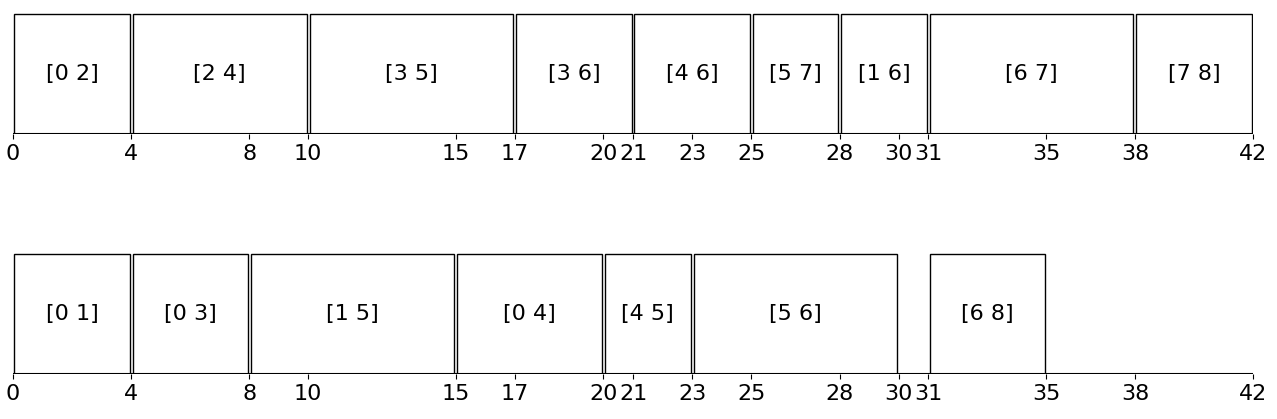
\includegraphics[width=0.95\textwidth]{diag4}
	\caption{Диаграмма Ганта. Критерий $max\ R$}
	\label{pic:diag4}
\end{center}
\end{figure}

Общее время работы: 42 часа.\  1-й простаивал 0 часов, 2-й --- 8 часов.\\[1cm]

Будем считать, что наилучшее расписание то, которое получено с использованием критерия наибольшего резерва ($max\ R$), потому что для него время простоя ресурсов оказалось минимальным, и время выполнения всех работ тоже оказалось минимальным. 

\end{document}